\begin{appendices}
    \chapter{Additional results} \label{app:additionalResults}
    \section{Validation plots} \label{app:verifResults}

    \begin{figure}[H]
    \centering
    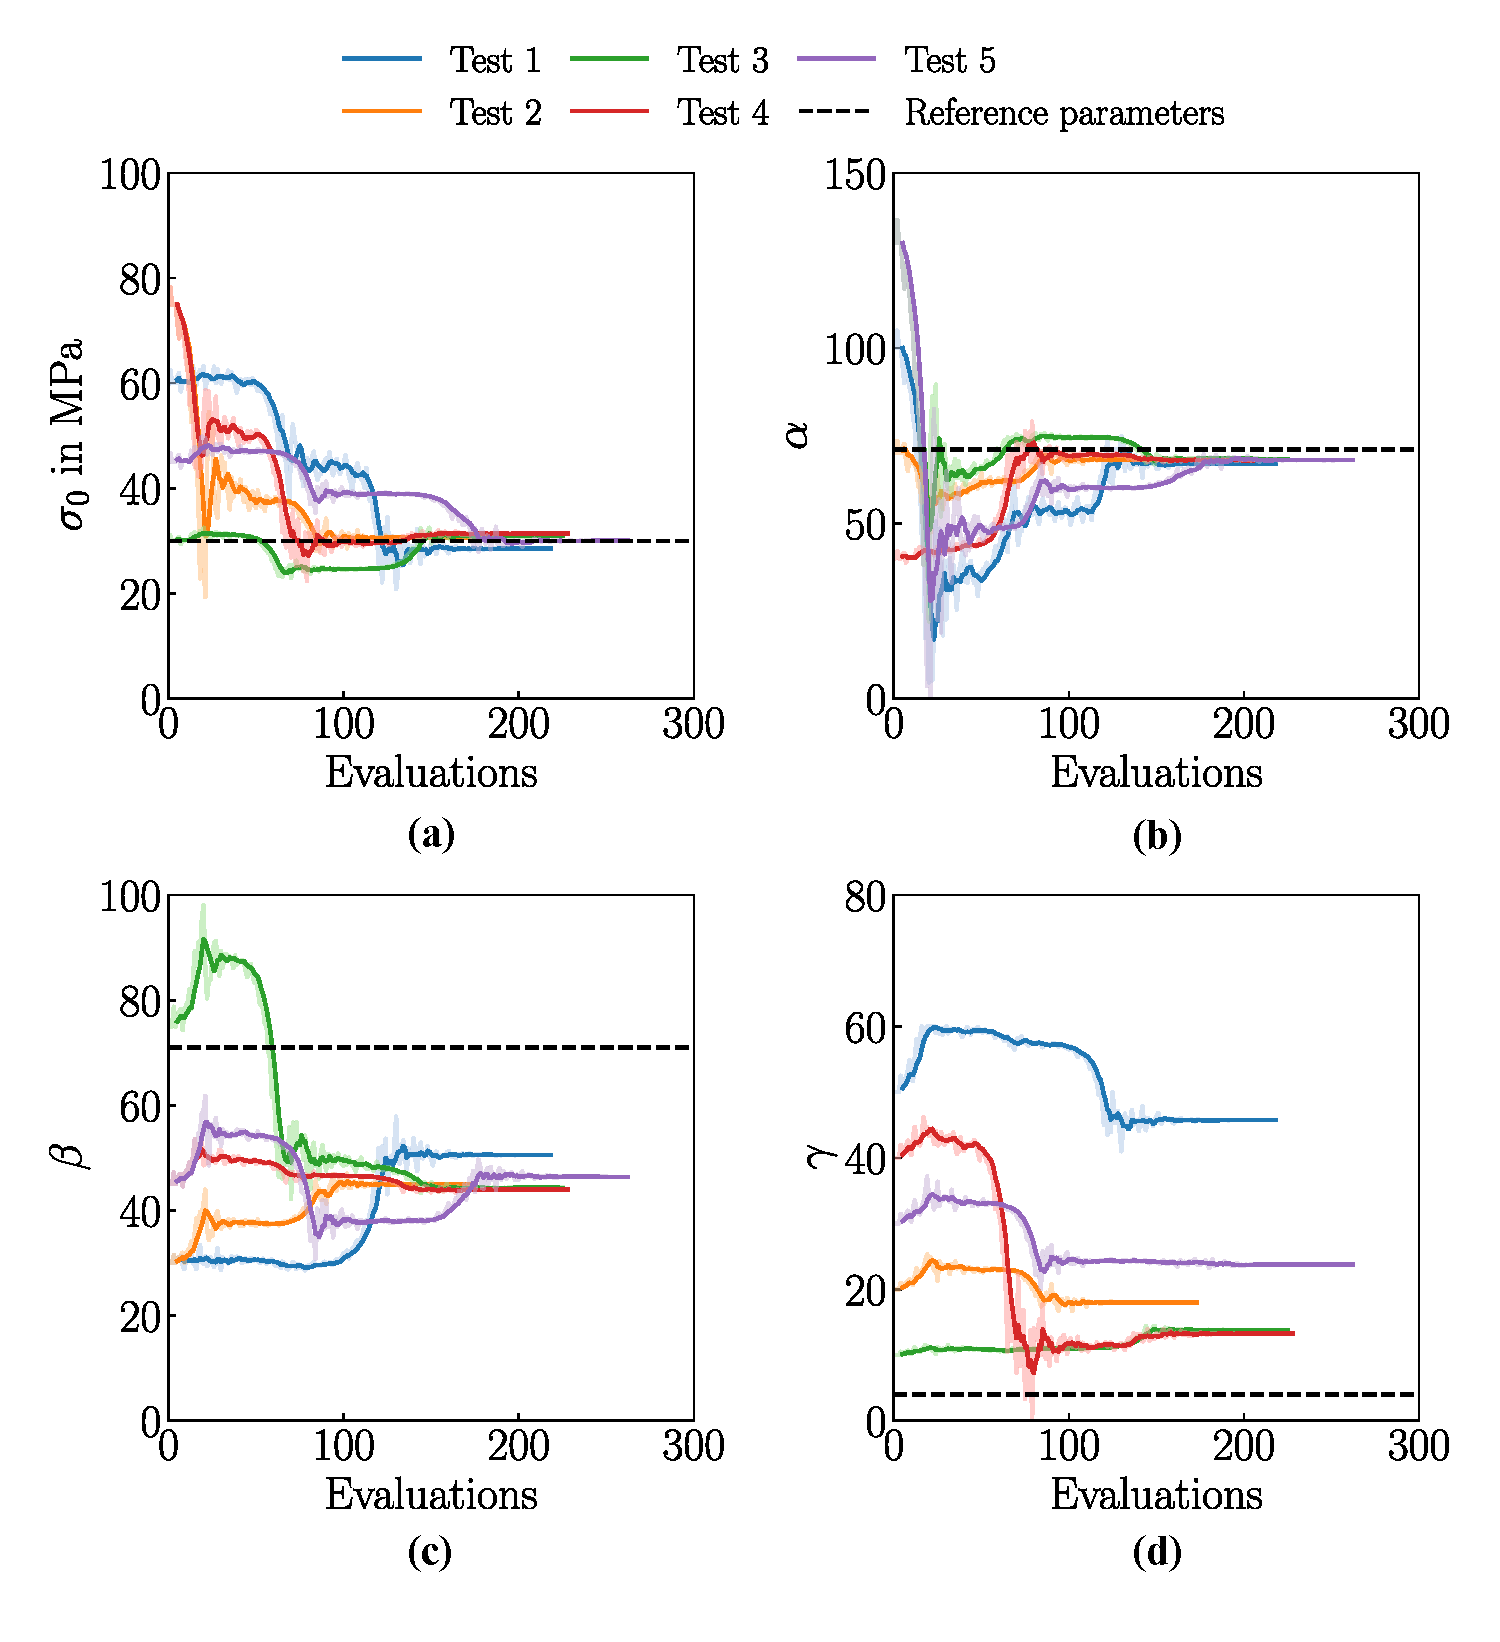
\includegraphics[width=0.66\textwidth]{Vald_4To3_fixEP1_material_params.pdf}
    \caption{Evolution of the optimised material parameters: (a) yield stress $\sigma_0$; hardening coefficients (b) $\alpha$; (c) $\beta$; (d) $\gamma$; over the optimisation evaluations for material with mixing ratio 4:3 under linear tensile strain with respective reference values obtained by \citet{ries_deciphering_nodate} and predefined elastic parameters Young's modulus $E$ and Poisson's ratio $\nu$}
    \label{fig:material_params_4to3}
    \end{figure}
    
    \begin{figure}[H]
    \centering
    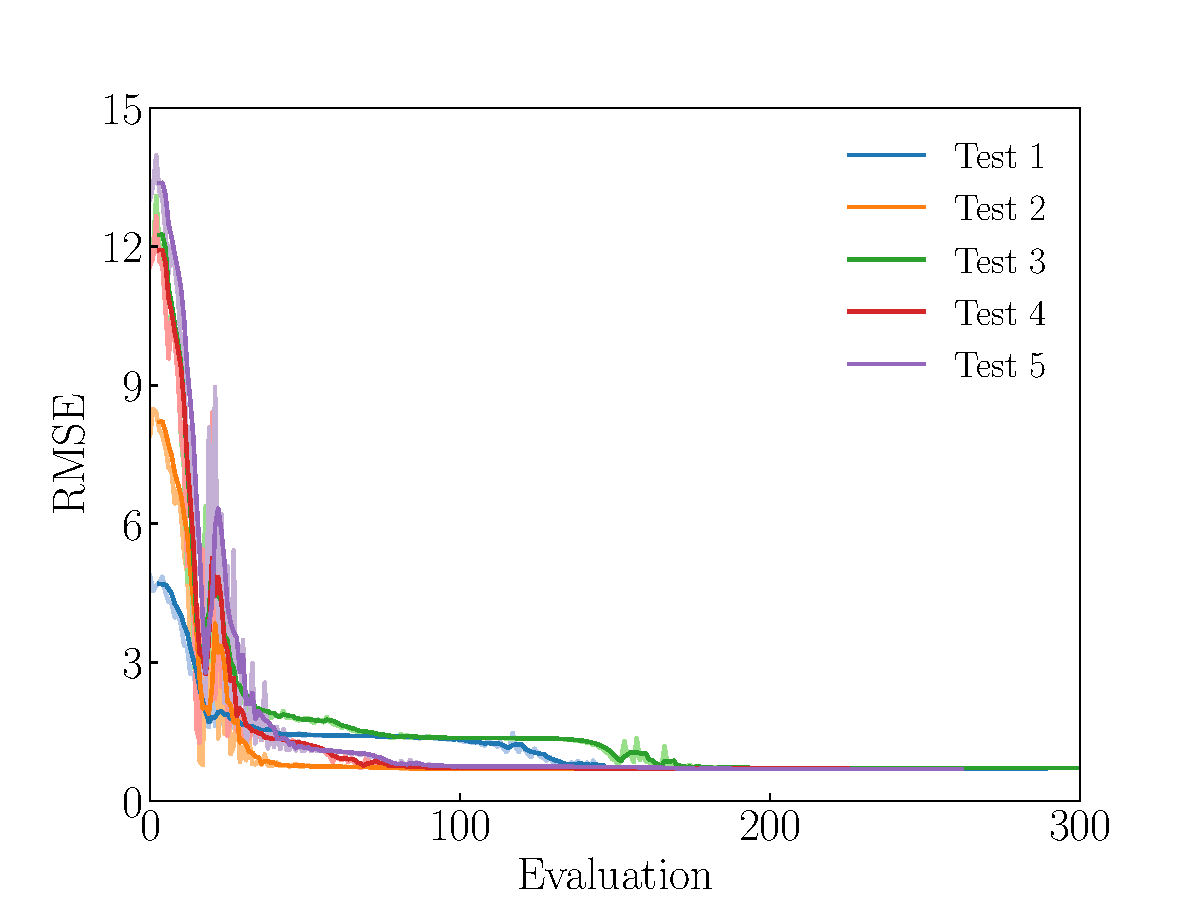
\includegraphics[width=0.5\textwidth]{Vald_4To3_fixEP1_rsme_lin_plot.pdf}
    \caption{Final \acrlong{olr} and \acrfull{rlr} $\varepsilon_{yy}$ over applied linear tensile strain $\varepsilon_{xx}$ for an exemplary test with material with mixing ratio 4:3 with predefined elastic parameters Young's modulus $E$ and Poisson's ratio $\nu$}
    \label{fig:strain_strain_4to3}
    \end{figure}

    \begin{figure}[H]
    \centering
    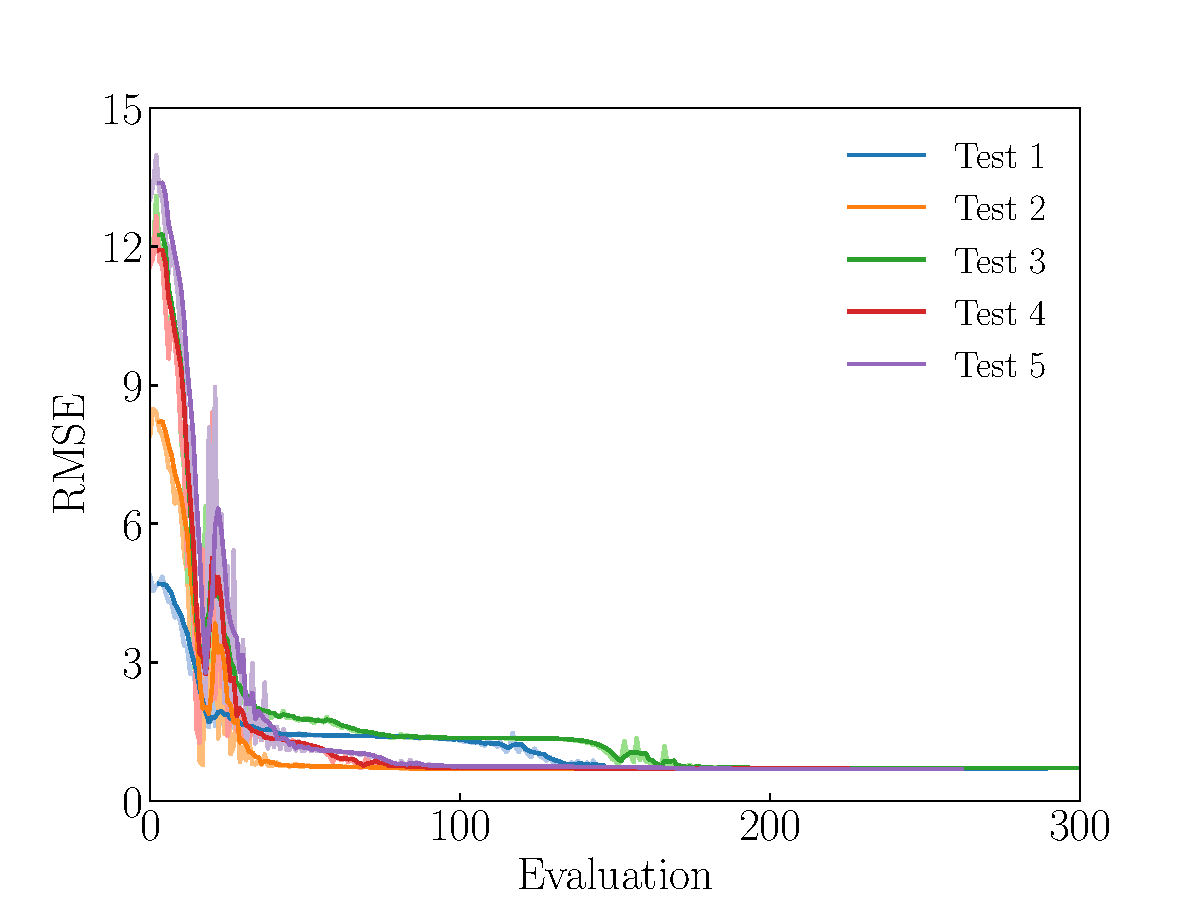
\includegraphics[width=0.5\textwidth]{Vald_4To3_fixEP1_rsme_lin_plot.pdf}
    \caption{Evolution of the \acrfull{rmse} during the optimisation for all tests for material with mixing ratio 4:3 under linear tensile strain}
    \label{fig:verfifRMSE43}
    \end{figure}

    \begin{figure}[H]
    \centering
    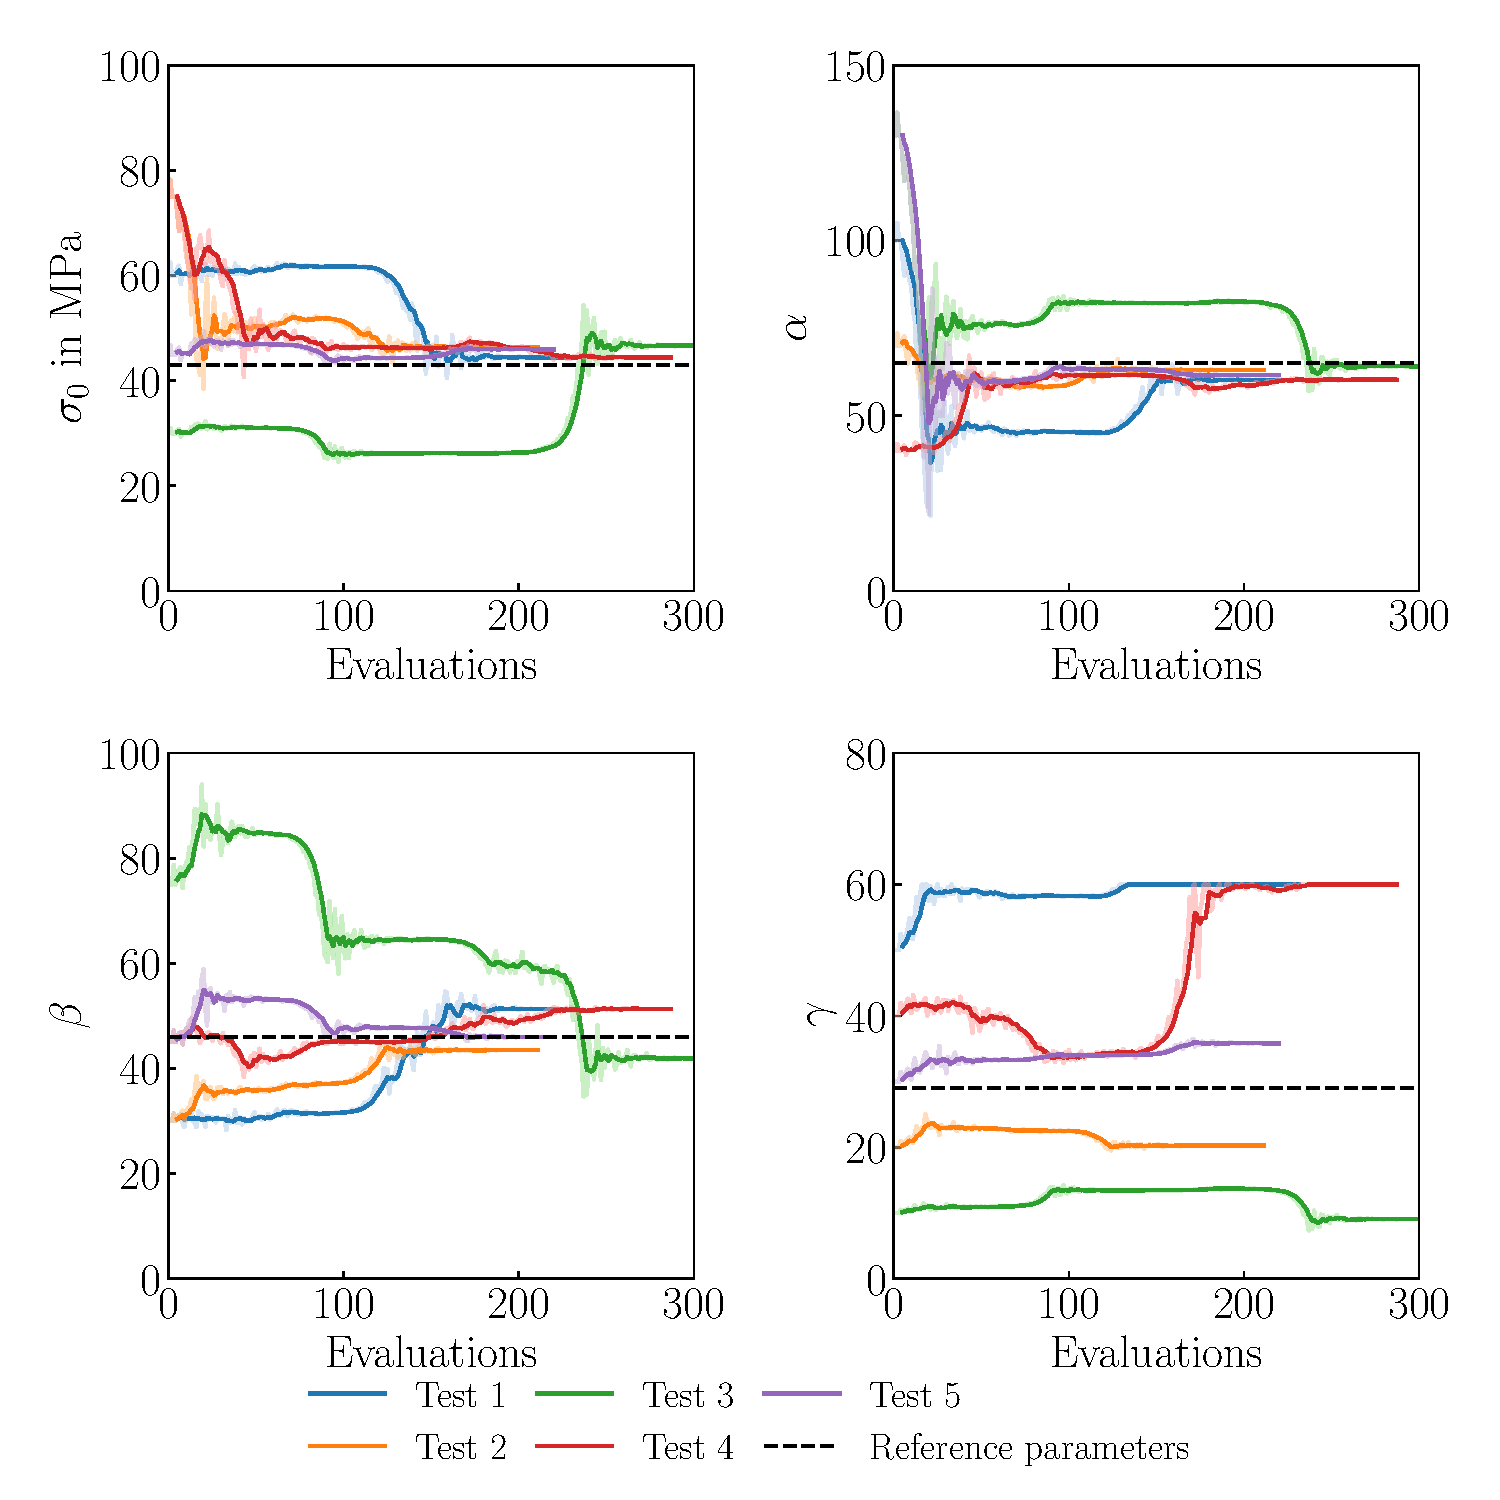
\includegraphics[width=0.66\textwidth]{Vald_8To3_fixEP1_material_params.pdf}
    \caption{Evolution of the optimised material parameters: (a) yield stress $\sigma_0$; hardening coefficients (b) $\alpha$; (c) $\beta$; (d) $\gamma$; over the optimisation evaluations for material with mixing ratio 8:3 under linear tensile strain with respective reference values obtained by \citet{ries_deciphering_nodate} and predefined elastic parameters Young's modulus $E$ and Poisson's ratio $\nu$}
    \label{fig:material_params_8to3}
    \end{figure}

    \begin{figure}[H]
    \centering
    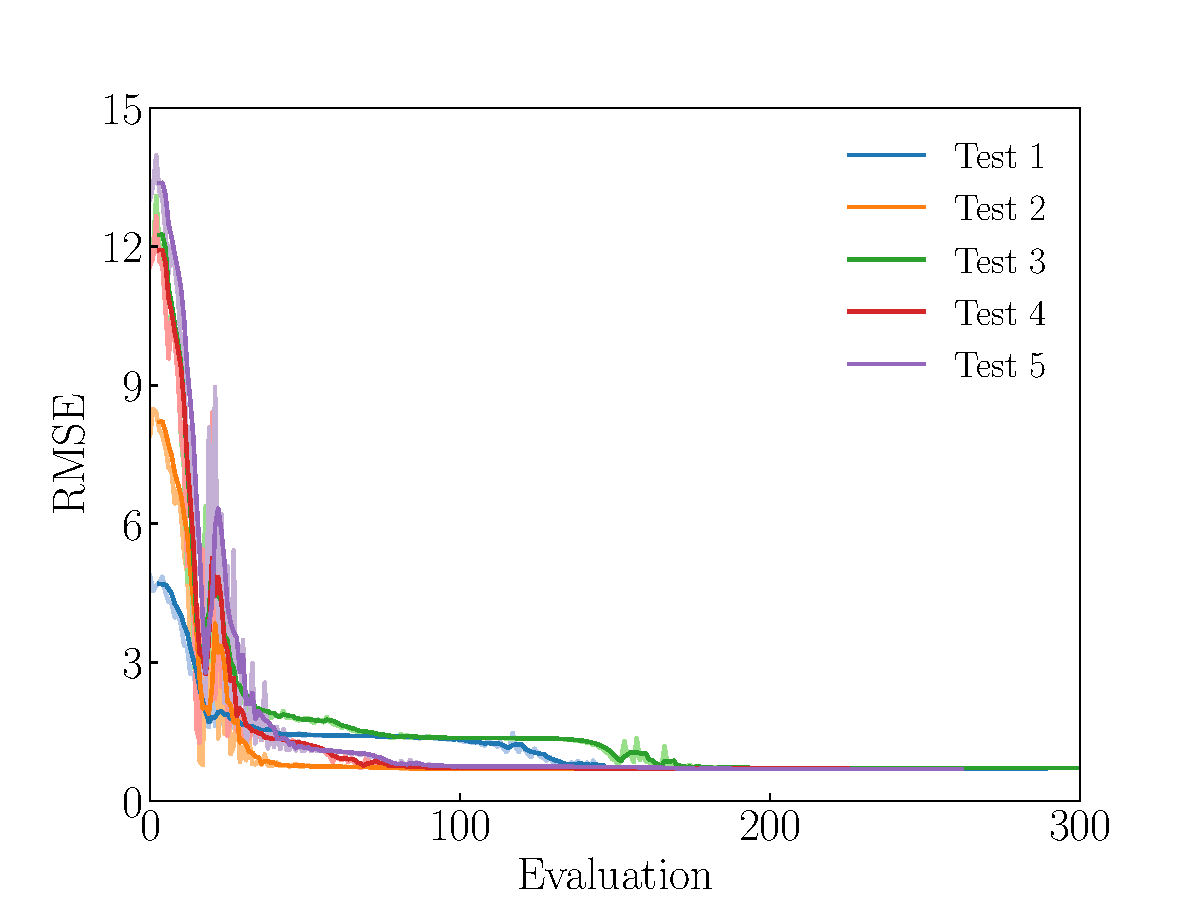
\includegraphics[width=0.5\textwidth]{Vald_4To3_fixEP1_rsme_lin_plot.pdf}
    \caption{Final \acrlong{olr} and \acrfull{rlr} $\varepsilon_{yy}$ over applied linear tensile strain $\varepsilon_{xx}$ for an exemplary test with material with mixing ratio 8:3 with predefined elastic parameters Young's modulus $E$ and Poisson's ratio $\nu$}
    \label{fig:strain_strain_8to3}
    \end{figure}

    \begin{figure}[H]
    \centering
    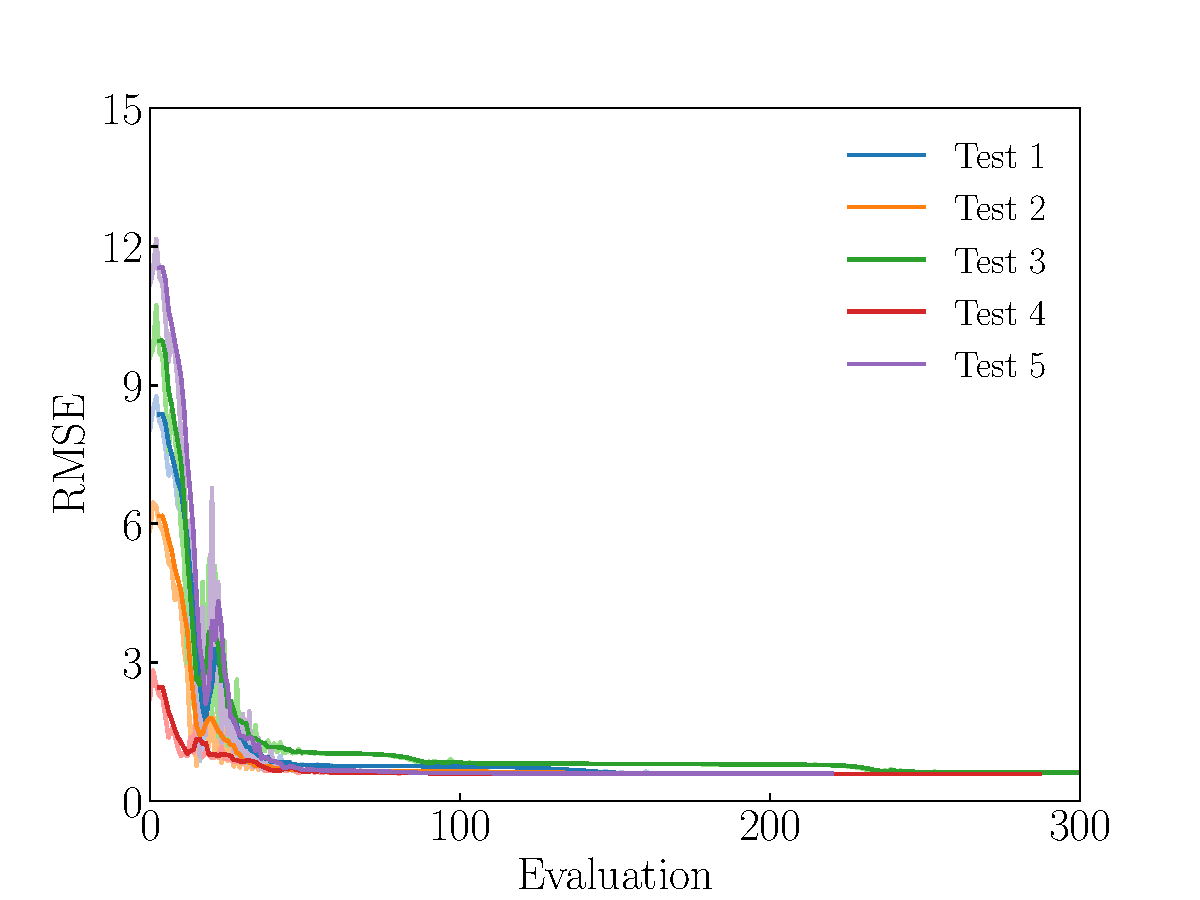
\includegraphics[width=0.5\textwidth]{Vald_8To3_fixEP1_rsme_lin_plot.pdf}
    \caption{Evolution of the \acrfull{rmse} during the optimisation for all tests for material with mixing ratio 8:3 under linear tensile strain}
    \label{fig:verfifRMSE83}
    \end{figure}


    \section{Tensile-Shear combination plots} \label{app:tensileShearResults}
    \begin{figure}[H]
    \centering
    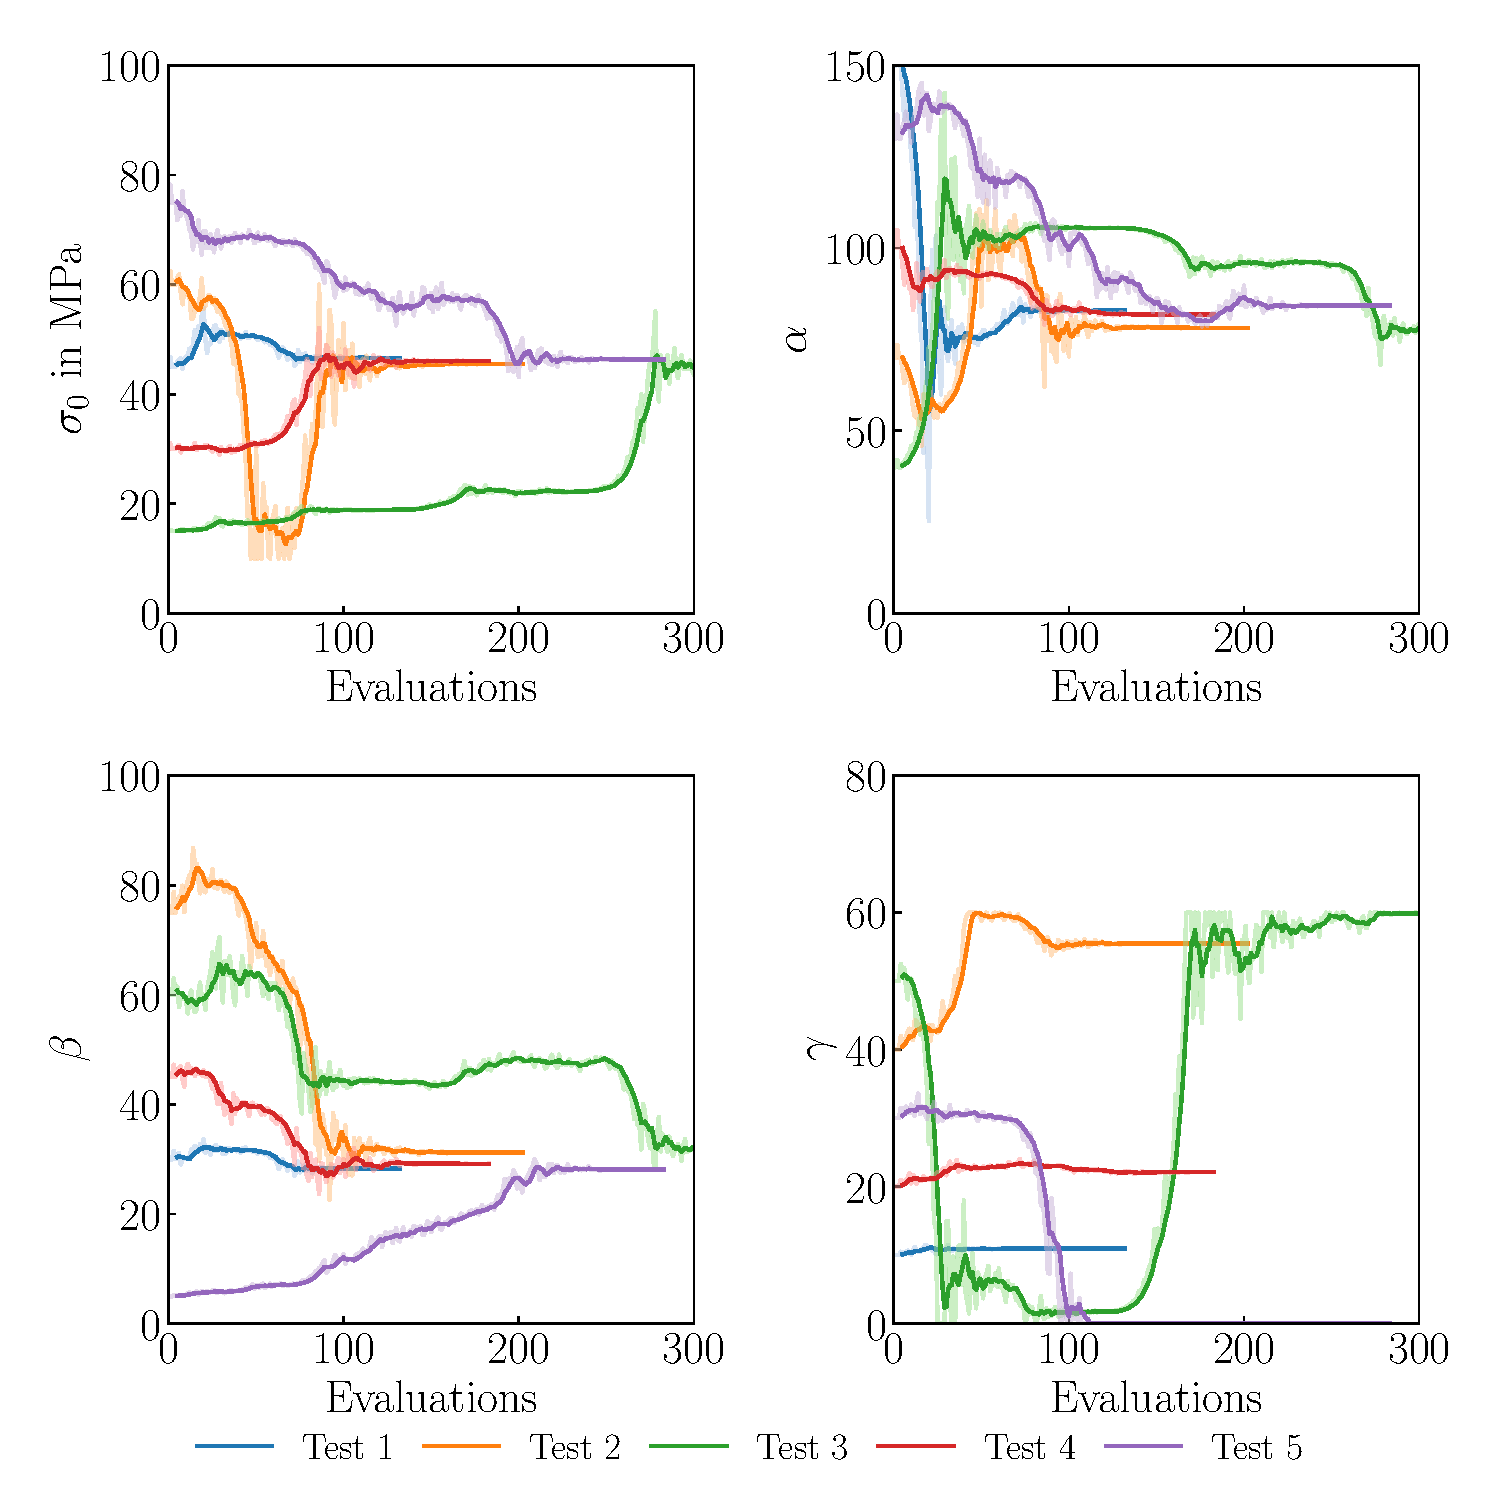
\includegraphics[width=0.7\textwidth]{Tensile_6to3_015_fixENu_material_params.pdf}
    \caption{Evolution of the optimised material parameters: (a) yield stress $\sigma_0$; hardening coefficients (b) $\alpha$; (c) $\beta$; (d) $\gamma$; over the optimisation evaluations for material with mixing ratio 6:3 under pure sinusoidal tensile strain and predefined elastic parameters Young's modulus $E$ and Poisson's ratio $\nu$}
    \label{fig:tensileMatParams}
    \end{figure}

    \begin{figure}[H]
    \centering
    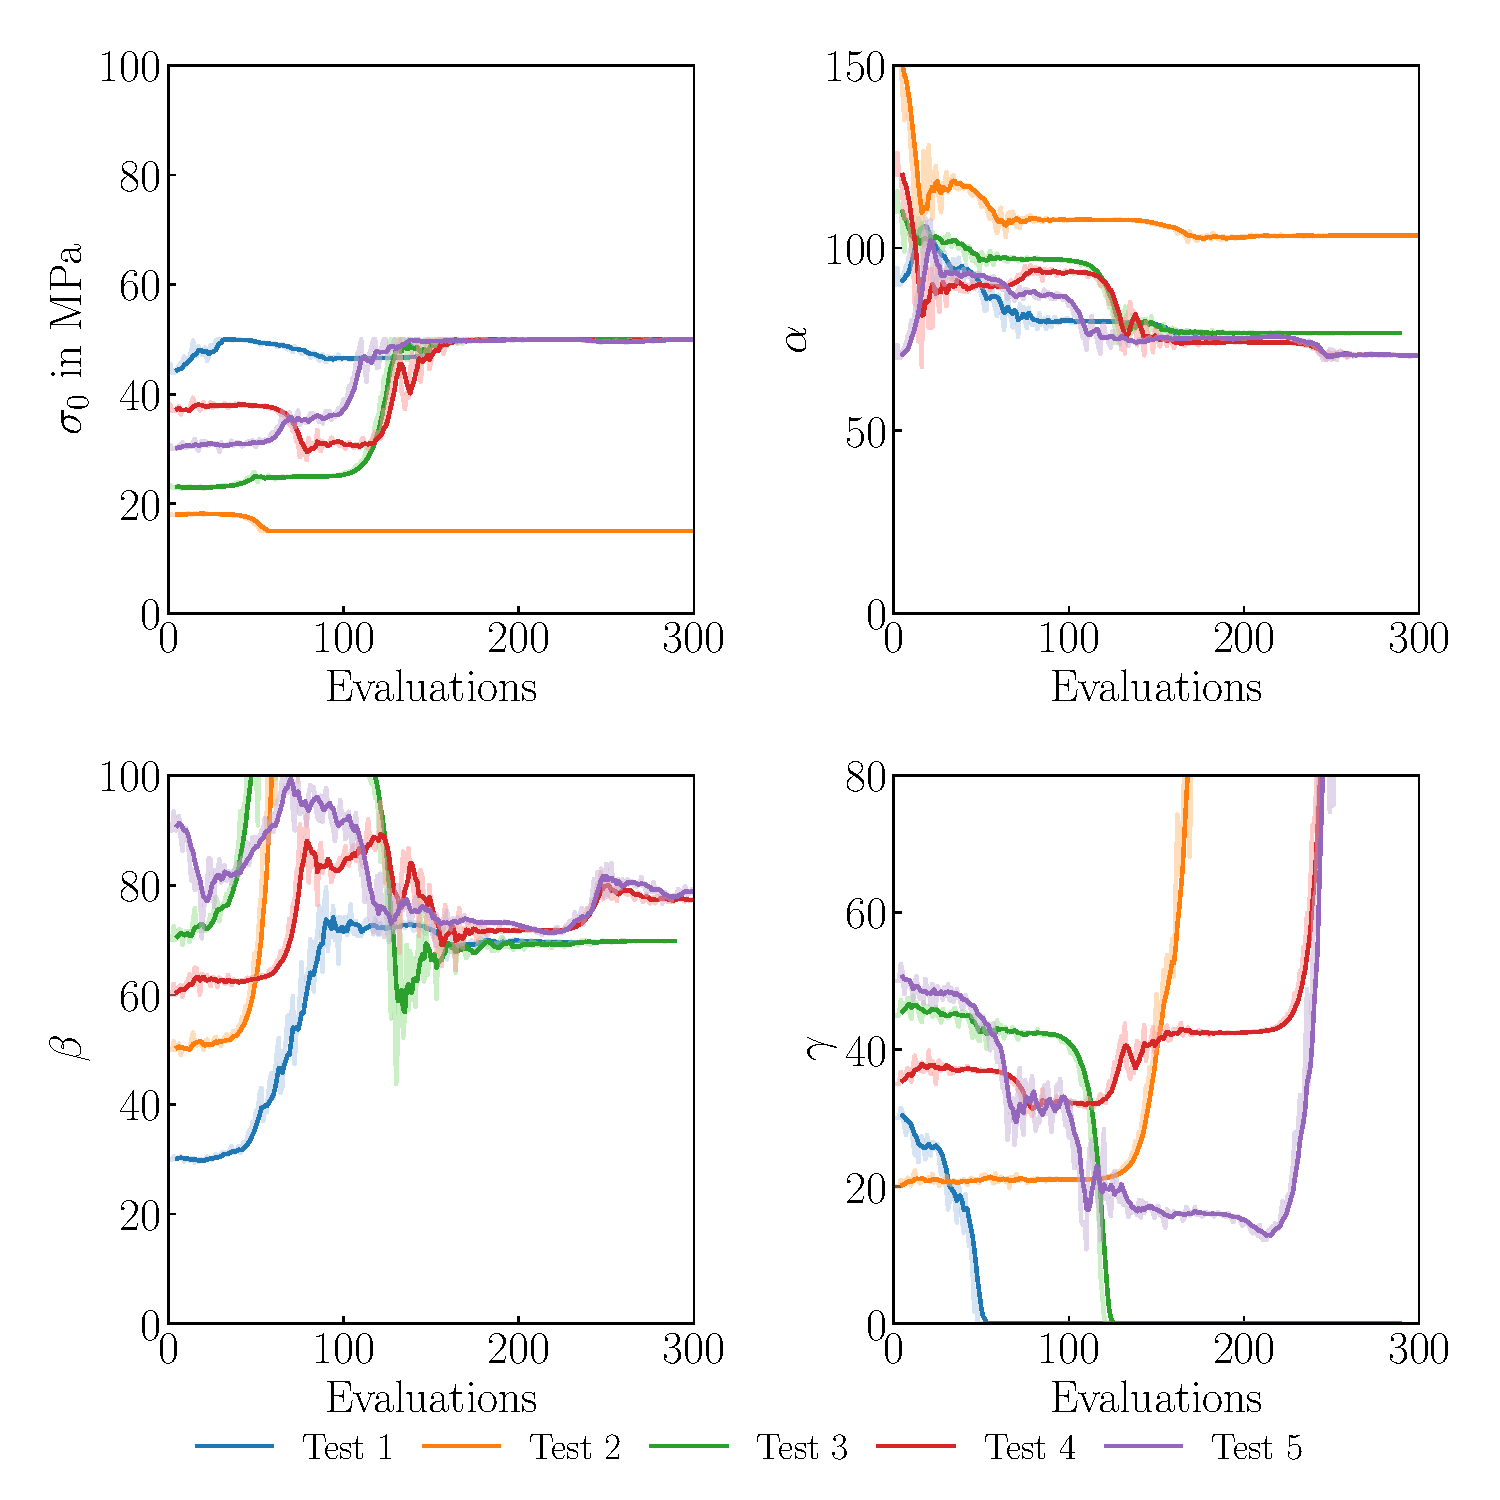
\includegraphics[width=0.7\textwidth]{Shear_6to3_015_fixENu_500_material_params.pdf}
    \caption{Evolution of the optimised material parameters: (a) yield stress $\sigma_0$; hardening coefficients (b) $\alpha$; (c) $\beta$; (d) $\gamma$; over the optimisation evaluations for material with mixing ratio 6:3 under pure sinusoidal shear strain and predefined elastic parameters Young's modulus $E$ and Poisson's ratio $\nu$}
    \label{fig:shearMatParams}
    \end{figure}


    XX STRAIN STRAIN FÜR VALIDIERUNGSVERSUCHE
    XX CODE UND INPUT FILE
    \chapter{Code} \label{app:Code}
    \section{Input file} \label{app:inputFile}

    \begin{lstlisting}[language=json,firstnumber=1]
    {   "Modelname": "Cube",
        "CubeSize": 1.0,
        "MaterialName": "CyclicMD",
        "MaterialType": "elasto-plastic",
        "YoungsModulus": {
            "value": [2500, 3000],
            "min": 2000, 
            "max": 4500
        },
        "PoissonRatio": {
            "value": [0.32, 0.38],
            "min": 0.23,
            "max": 0.45
        },
        
        "PlasticYield": {
            "value": [50.0, 35.0],
            "min": 10.0,
            "max": 100.0
        },
        "Alpha": {
            "value": [100.0, 70.0],
            "min": 0.0,
            "max": 200.0
        },
        "Beta": {
            "value": [45.0, 20.0],
            "min": 0.0,
            "max": 100.0
        },
        "Gamma": {
            "value": [10.0, 40.0],
            "min": 0.0,
            "max": 60.0
        },
        "C10": {
            "min": 310.0,
            "max": 650.0
        },
        "D1": {
            "min": 0.00018,
            "max": 0.0018
        },
        "PlasticMaterialParameters": "voce.dat",
        "NumberOfElementsPerEdge": 6,
        "MDDataFiles": [
            {"filename": "exemplary_reference_data.dat", "weight": 1.0}
        ],
        "PrescribedDirections": { 
            "E11": {"active": 1, "weight": 1.0},
            "E22": {"active": 0, "weight": 0.0},
            "E33": {"active": 0, "weight": 0.0},
            "G12": {"active": 1, "weight": 1.0},
            "G13": {"active": 0, "weight": 0.0},
            "G23": {"active": 0, "weight": 0.0}
        },
        "StressAnalysisDirection": {
            "xx": 1,
            "yy": 0,
            "zz": 0,
            "xy": 1,
            "xz": 0,
            "yz": 0
        },
        "StrainAnalysisDirection": {
            "xx": 0,
            "yy": 1,
            "zz": 1,
            "xy": 0,
            "xz": 0,
            "yz": 0
        },
        "weights": {
            "normalStress": 1,
            "normalStrain": 1e4,
            "shearStress": 1,
            "shearStrain": 1e30
        },
        "NumberOfIterations": 300,
        "Testname": "tensile_shear_combi_test"
    }

    \end{lstlisting}
    \newpage
    \section{Optimisation algorithm}\label{app:Script}
    \lstinputlisting[language=Python]{Optimization_complete_cyclic.py}
\end{appendices}